\section{Derivation of the repeated-branch diagnostic}
\label{app:proof}

For a fixed task, write $m^{(r)}=\max_aY_a^{(r)}$ and $\widehat a^{(r)}=\arg\max_aY_a^{(r)}$, breaking ties by the lowest action index. Because $a=0$ carries the lowest index, continuation wins every tie in which it attains the maximum, and the lowest-indexed successful intervention wins otherwise. This convention fixes the realized value of $G$ in the binary-outcome case, where ties are common. For either draw,
\begin{equation}
m^{(0)}-Y_{\widehat a^{(1)}}^{(0)}\geq0,
\qquad
m^{(1)}-Y_{\widehat a^{(0)}}^{(1)}\geq0,
\end{equation}
because the selected action from the other draw remains an element of the maximization set. Their mean is $G$, so $G\geq0$ pathwise. The result is unchanged by ties because any deterministic tie choice indexes an available action.

Now condition on the shared prefix $X=x$. Let the two action-outcome vectors be independent and identically distributed given $X=x$; independence is what allows the cross-draw term to factor, and identical distribution is what makes the two orderings interchangeable. Then
\begin{align}
\mathbb E[G\mid x]
&=\mathbb E[m^{(0)}\mid x]
-\mathbb E[Y_{\widehat a^{(1)}}^{(0)}\mid x] \\
&=\mathbb E\!\left[\max_aY_a\mid x\right]
-\mathbb E\!\left[\mu_{\widehat a(Y')} (x)\mid x\right],
\end{align}
where $Y'$ is an independent action-outcome vector and $\widehat a(Y')$ is the action selected from it. The first term is a realized maximum. The second is the value of the outcome-informed selection rule on a fresh continuation. It is not the value of any prefix-only deployable controller. If all actions share the same success probability but outcomes fluctuate, the difference may still be positive; $G$ therefore identifies evaluation optimism rather than a causal intervention effect.

Two consequences follow for inference. First, a sign-flip permutation null is degenerate for $G$: non-negativity makes every group sum non-negative, the observed statistic is the algebraic maximum over sign vectors, and rejection only excludes deterministic continuations. We therefore report $G$ as an estimate with bootstrap intervals and exclude it from the tested family. Second, the mechanical part of $G$ can be quantified directly. Permuting the recorded outcomes within a task across all action and draw cells holds the number of successes fixed, preserves the continuation noise level, and destroys any action structure. The mean of $G$ under this within-task permutation is the noise floor that a homogeneous menu would produce, and the observed $G$ is read against it. With $R>2$ draws we average $G$ over ordered draw pairs, which reduces to Equation~\ref{eq:gap} at $R=2$.

\section{Action and information contracts}
\label{app:actions}

\begin{table}[ht]
\caption{The complete frozen action menu. Arms 0--3 are the first confirmation's contract, unchanged; arms 4 and 5 are added by the second confirmation. The message is inserted once immediately before the next actor decision and remains in the visible transcript.}
\label{tab:messages}
\centering
\small
\begin{tabular}{@{}clp{0.66\linewidth}@{}}
\toprule
Arm & Name & Operation \\
\midrule
0 & \textsc{Continue} & Restore the checkpoint and append no message. \\
1 & \textsc{Warning} & ``Re-check the goal, the latest observation, and your previous action. Continue only after correcting any inconsistency you notice.'' \\
2 & \textsc{Replan} & ``Construct a fresh, concise plan from the current goal and observable state. Then execute that plan.'' \\
3 & \textsc{Rollback--replan} & Restore the serialized environment and dialogue state at step $t-1$, append ``The previous attempted action has been reverted. Construct a fresh, concise plan from the current goal and restored observable state. Then execute that plan,'' and set the suffix limit to $L-1$. \\
4 & \textsc{Deep rollback--replan} & Restore the serialized environment and dialogue state at step $t-3$, clamped at the episode start, append ``Your three most recent decisions have been reverted and the environment restored to the state before them. Construct a fresh, concise plan from the current goal and restored observable state. Then execute that plan,'' and set the suffix limit to $L-k$ for the $k$ reverted decisions. \\
5 & \textsc{Locate} & ``Before acting again, name the objects this task still requires and the places you have not yet inspected. Then inspect the most promising place.'' \\
\bottomrule
\end{tabular}
\end{table}

Every arm receives the same task instruction, public action history, public observations, actor weights, decoding parameters, and total decision budget. An arm that reverts $k$ decisions restores the serialized snapshot at step $t-k$ unconditionally, regardless of domain-level physical reversibility, and receives suffix limit $L-k$ for an episode limit $L$; the actor therefore makes exactly $L$ decisions on every arm and $L-k$ environment actions remain in the episode. The controller receives only fields computed from the prefix. Environment state hashes, future observations, suffix outcomes, rollback metadata, and task-selection provenance are excluded. Arm 3 has no special access to a future legal-action sequence. The intervention decision occurs once per episode.

\section{Controller construction and development selection}
\label{app:controller}

The 50 numeric features are action-class fractions; counts and rates of admissible, repeated, invalid, and failed actions; reward summaries; observation and prompt lengths; token usage; action and observation novelty; vocabulary growth; and step index. Environment and checkpoint identity enter through the stratum: a separate forest is fitted for each actor and environment, and the checkpoint index is one of the 50 numeric fields. No categorical task identifier is encoded. The text field concatenates the recent public observations and actions. Word TF--IDF uses a vocabulary of at most 512 terms, and the resulting representation is reduced to at most 16 truncated-SVD components. All text fitting occurs inside each task-group fold during development selection. The final transform is refit on all admitted development tasks only.

\begin{table}[ht]
\caption{Development-only policy selection for the first confirmation; the admitted development task count per environment is given in parentheses. Utilities average the two saved continuation draws within each complete task row. The strongest matched comparator and the operational selection were fixed before confirmation outcomes.}
\label{tab:development}
\centering
\small
\begin{tabular}{@{}llrr@{}}
\toprule
Environment & Candidate & OOF utility (\%) & Intervention rate (\%) \\
\midrule
\multirow{5}{*}{ALFWorld (129)}
& \textsc{Continue} & 45.35 & 0.00 \\
& \textsc{Best fixed} (arm 2) & 50.39 & 100.00 \\
& \textsc{Direct} & 47.67 & 34.11 \\
& \textsc{Arm outcome} (\textsc{Repeated}) & 47.29 & 96.90 \\
& \textsc{Single-1} & \textbf{51.16} & 79.84 \\
\midrule
\multirow{5}{*}{ScienceWorld (55)}
& \textsc{Continue} & 20.91 & 0.00 \\
& \textsc{Best fixed} (arm 2) & 24.55 & 100.00 \\
& \textsc{Direct} & 23.64 & 21.82 \\
& \textsc{Arm outcome} (\textsc{Repeated}) & 23.64 & 89.09 \\
& \textsc{Single-1} & \textbf{27.27} & 100.00 \\
\bottomrule
\end{tabular}
\end{table}

The repeated arm-outcome control, \textsc{Repeated}, predicts all four outcomes after fitting to the mean of two draws. \textsc{Single-1} uses the same action-outcome formulation but fits to one predesignated draw; it was the strongest runnable development comparator. \textsc{Direct} predicts three outcomes relative to continuation. Both target-parameterization learners share the same feature builder, task-group folds, 200-tree random-forest class, minimum-leaf grid $\{5,10\}$, continuation-margin grid $\{0.00,0.05,0.10\}$, and task rows. A candidate must exceed the continuation margin to intervene; otherwise it chooses arm 0. \textsc{Cross-draw} fits one signed-benefit forest per development draw on the same folds, features, and capacity, and adds two entries to the shared grid: an agreement requirement and a restriction of the candidates to the two arms with the highest mean benefit inside the training fold. With agreement required, it fires the common arm $\widehat a^{(0)}=\widehat a^{(1)}$ when the mean of the two cross-draw values exceeds the margin, and declines otherwise; this rule performs no maximization over scores that also value the chosen arm. Without agreement required, it keeps the better of the two cross-scored candidates, which is a maximization over two honestly cross-scored values rather than over the full menu. Both entries are scored by development out-of-fold utility inside the same frozen grid, and the candidate set is recomputed inside every training fold. We additionally report a nested out-of-fold utility that selects leaf, margin, and both added entries inside each training fold and scores the resulting rule on the held-out fold, which removes the optimism of selecting and scoring a grid on the same folds. Utility ties favor the fallback that the nested inner folds chose most often, then the lower firing rate, then the prespecified candidate order.

\section{Panel construction and lineage}
\label{app:lineage}

The ALFWorld source inventory was grouped by its six task types. We removed every goal directory found in the 59 supplied prior configuration and outcome files, ranked the remaining identities by SHA-256 with seed 270914, and retained the first 64 identities per type. The resulting 384 tasks occupy 96 floorplan groups. ScienceWorld began from a 57-variation reserved official-test frame. We verified that none of its variations occurred among the 227 variations in the supplied exposure packet; the panel occupies 25 task families. These exclusions establish independence from the supplied research record, not from model pretraining or all work by other parties.

The second study draws from the same inventory after removing, in addition, every goal directory used by the first confirmation panel. Its confirmation panel holds 288 identities balanced across the six task types; its development panel holds 424 further identities and is disjoint from both confirmation panels. The two checkpoint rules run the same 288 confirmation identities, so the rule contrast is paired at the task level; because the frozen configuration hash differs between the rules, each rule generates its own baseline episode under the same task specification, seed, actor revision, and decoding parameters.

\begin{table}[ht]
\caption{Pre-outcome lineage. Full digests are machine-checked in the supplement.}
\label{tab:lineage}
\centering
\small
\begin{tabular}{@{}lp{0.69\linewidth}@{}}
\toprule
Object & Frozen identifier \\
\midrule
Panel and analysis commit & \texttt{8ddf66b} and \texttt{4dd0785} precede baseline generation \\
Prediction-freeze commit & \texttt{f0f26bf}, pushed before arm generation \\
Eligible prefixes & 406: 355 ALFWorld and 51 ScienceWorld \\
Prefix digest & \texttt{0f5a80d1...46e863} \\
Prediction digest & \texttt{78380914...f6911b} \\
Arm-outcome family bundle digest & \texttt{759b9d02...7d612b}; it holds every arm-outcome learner, including \textsc{Repeated} and the selected \textsc{Single-1} \\
Direct model digest & \texttt{4ad68910...fe16db} \\
\bottomrule
\end{tabular}
\end{table}

Baseline generation produced 35 structural early terminations. One episode exceeded its original coordinator lease. A single administrative resume reused the frozen task, seed, actor, software, and checkpoint rule; the interrupted attempt and resumed occupancy are both retained in the append-only ledger. No arm outcome was available when features and actions for the remaining 406 prefixes were serialized and committed. During arm generation, eight serving endpoints became unavailable after roughly one hour, leaving 560 canonical cells with technical failure flags. The evaluator rejected that state. The administrative resume archived every failed cell as an \texttt{attempt1} record and regenerated only those cells with their original configuration, prefix, action, draw, and request seeds. A separate server preflight failed on an occupied port and generated no outcome; restarting it on a different port completed the shard. No second-attempt record exists, and no failed cell enters the analysis.

\section{Complete statistical specification}
\label{app:statistics}

For a policy $p$, task-level utility is the mean of the two selected arm outcomes. Structural early-terminal tasks contribute their observed terminal success to every policy. A policy contrast is the paired difference in task utility. Task-bootstrap intervals resample tasks with replacement. Group-bootstrap intervals resample floorplans for ALFWorld and task families for ScienceWorld, retaining every task in each sampled group. Both use 10,000 draws and fixed stored seeds.

The primary randomization statistic is the absolute mean task contrast. Under the null, we independently multiply each group sum by $-1$ or $+1$, retaining within-group task dependence, and compare 50,000 Monte Carlo assignments with the observed statistic. The Monte Carlo $p$ value includes the observed assignment through the usual plus-one correction. We order the raw ALFWorld $p$ values within a family and apply Holm's step-down adjustment. The first confirmation's family comprises the optimism gap, \textsc{Direct} minus \textsc{Continue}, and \textsc{Direct} minus \textsc{Single-1}; the second confirmation's family comprises \textsc{Cross-draw} minus \textsc{Continue} and \textsc{Cross-draw} minus the development-best unconditional action, and collapses to the first of these when that action is continuation. The evaluator records the family it applied. All other tests and intervals are descriptive secondary analyses.

Recoveries count draw-level cases in which continuation fails and the policy succeeds. Disruptions count the reverse. Intervention rate is computed over eligible prefixes; success denominators include all planned tasks. Request, token, and client-wall-time summaries report the selected suffix for eligible tasks. The release additionally preserves all recorded calls and the GPU lease ledger. No missing eligible cell is imputed: the final evaluator refuses to emit results if any required arm-by-draw cell is absent.

\section{Complete confirmation results}
\label{app:results}

ScienceWorld provides a prespecified boundary rather than a second opportunity to claim success. Its continuation success rate is 19.30\%, so most tasks fail under every action and contribute zero to both the gap and every contrast; the panel therefore compresses effects mechanically rather than showing greater branch stability. Its same-draw gap is 5.26 points ([1.69, 10.00] by task-family bootstrap), and Direct minus Continue is 0.00 points; its [0.00, 0.00] interval is degenerate because the controller fired on 11.8\% of prefixes and produced no recovery or disruption, which is an absence of observed differences rather than an exact null. All 57 tasks, 25 families, six policies, costs, recoveries, and disruptions appear in Table~\ref{tab:scienceworld-contrasts} and the released result JSON. Differences in direction across environments narrow the empirical scope instead of motivating post hoc domain selection.


\begin{table}[ht]
\caption{Complete confirmation policy census. Success uses every planned task. Firing is over eligible prefixes; recoveries and disruptions count the two draw-level comparisons with continuation.}
\label{tab:confirmation-policies}
\centering
\small
\begin{tabular}{@{}llrrrr@{}}
\toprule
Domain & Policy & Success (\%) & Fire (\%) & Recover & Disrupt \\
\midrule
\multirow{6}{*}{ALFWorld} & Continue & 52.86 & 0.0 & 0 & 0 \\
 & Best fixed & 55.34 & 100.0 & 74 & 55 \\
 & Direct & 54.43 & 31.0 & 26 & 14 \\
 & Arm outcome & 54.04 & 96.6 & 69 & 60 \\
 & Matched & 54.82 & 78.0 & 66 & 51 \\
 & Safe selected & 54.82 & 78.0 & 66 & 51 \\
\midrule
\multirow{6}{*}{ScienceWorld} & Continue & 19.30 & 0.0 & 0 & 0 \\
 & Best fixed & 19.30 & 100.0 & 5 & 5 \\
 & Direct & 19.30 & 11.8 & 0 & 0 \\
 & Arm outcome & 19.30 & 100.0 & 5 & 5 \\
 & Matched & 14.04 & 100.0 & 2 & 8 \\
 & Safe selected & 14.04 & 100.0 & 2 & 8 \\
\bottomrule
\end{tabular}
\end{table}

Figure~\ref{fig:effects} shows both marginal task and grouped uncertainty for the primary family and the selected deployment rule. The group intervals are wider whenever shared floorplans induce material composition sensitivity. Statistical significance is determined only by the frozen group sign-flip family, not by whether a plotted interval excludes zero.

\begin{figure}[ht]
\centering
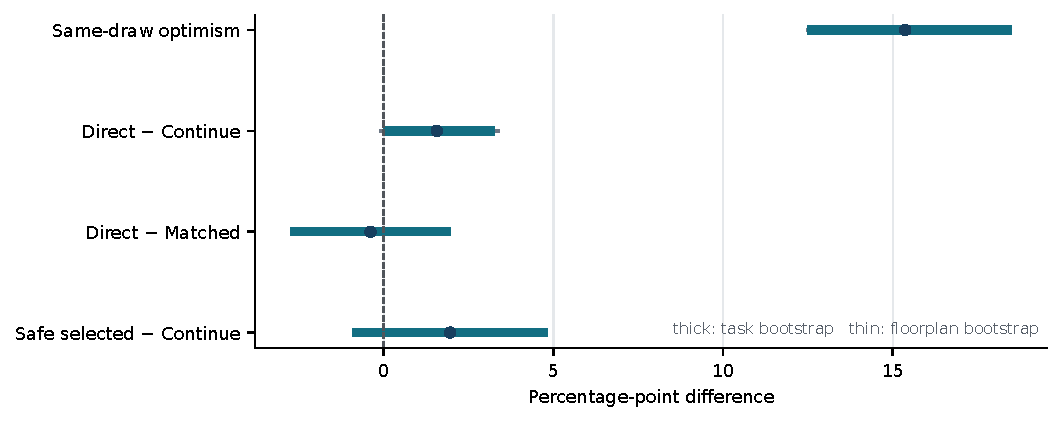
\includegraphics[width=\linewidth]{figures/policy-effects.pdf}
\caption{Confirmation effects on ALFWorld. Dots show planned-task means; thick and thin intervals show task- and floorplan-bootstrap 95\% intervals. Reported adjusted $p$ values use the prespecified group sign-flip tests and Holm correction.}
\label{fig:effects}
\end{figure}


\begin{figure}[ht]
\centering
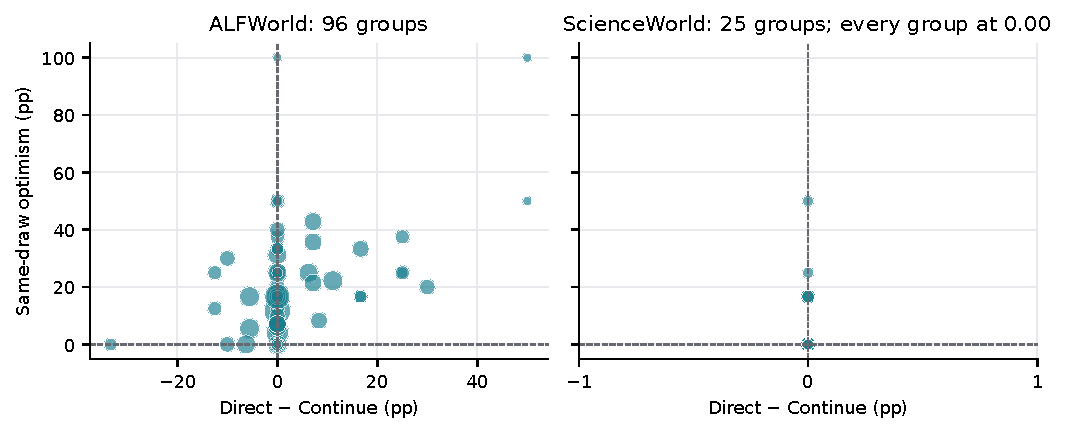
\includegraphics[width=\linewidth]{figures/group-results.pdf}
\caption{Group-level measurement and policy effects. Each point is a complete floorplan or task-family group; area is proportional to its task count. Vertical position is same-draw optimism and horizontal position is Direct minus Continue. Dashed lines mark zero.}
\label{fig:groups}
\end{figure}



\begin{table}[ht]
\caption{All ALFWorld contrasts. Values are percentage points. Holm adjustment applies only to the first two rows and the same-draw diagnostic in the text.}
\label{tab:alfworld-contrasts}
\centering
\scriptsize
\begin{tabular}{@{}lrrrrr@{}}
\toprule
Contrast & Mean & Task 95\% & Group 95\% & Group $p$ & Holm $p$ \\
\midrule
Direct $-$ Continue & 1.56 & [0.00, 3.26] & [\ensuremath{-0.12}, 3.41] & 0.1048 & 0.2096 \\
Direct $-$ Matched & \ensuremath{-0.39} & [\ensuremath{-2.73}, 1.95] & [\ensuremath{-2.26}, 1.57] & 0.7927 & 0.7927 \\
Direct $-$ Arm outcome & 0.39 & [\ensuremath{-2.21}, 2.99] & [\ensuremath{-1.82}, 2.64] & 0.8228 & -- \\
Direct $-$ Best fixed & \ensuremath{-0.91} & [\ensuremath{-3.39}, 1.56] & [\ensuremath{-3.09}, 1.31] & 0.4881 & -- \\
Safe selected $-$ Continue & 1.95 & [\ensuremath{-0.91}, 4.82] & [\ensuremath{-0.38}, 4.26] & 0.1311 & -- \\
\bottomrule
\end{tabular}
\end{table}

\begin{table}[ht]
\caption{All ScienceWorld contrasts, retained as unadjusted boundary analyses. Values are percentage points.}
\label{tab:scienceworld-contrasts}
\centering
\scriptsize
\begin{tabular}{@{}lrrrrr@{}}
\toprule
Contrast & Mean & Task 95\% & Group 95\% & Group $p$ & Holm $p$ \\
\midrule
Direct $-$ Continue & 0.00 & [0.00, 0.00] & [0.00, 0.00] & 1.0000 & -- \\
Direct $-$ Matched & 5.26 & [\ensuremath{-0.88}, 12.28] & [\ensuremath{-0.81}, 11.86] & 0.1860 & -- \\
Direct $-$ Arm outcome & 0.00 & [\ensuremath{-5.26}, 5.26] & [\ensuremath{-4.17}, 4.39] & 1.0000 & -- \\
Direct $-$ Best fixed & 0.00 & [\ensuremath{-5.26}, 5.26] & [\ensuremath{-4.17}, 4.39] & 1.0000 & -- \\
Safe selected $-$ Continue & \ensuremath{-5.26} & [\ensuremath{-12.28}, 0.88] & [\ensuremath{-11.86}, 0.81] & 0.1860 & -- \\
\bottomrule
\end{tabular}
\end{table}

ALFWorld same-draw optimism is 15.36 percentage points with task-bootstrap interval [12.50, 18.49], group-bootstrap interval [12.46, 18.30], raw group sign-flip $p=<10^{-4}$, and Holm-adjusted $p=<10^{-4}$. These preregistered $p$ values are retained for audit; the nonnegative gap makes their symmetric null scientifically narrow, and they are not tests of intervention benefit. ScienceWorld optimism is 5.26 percentage points with task-family-bootstrap interval [1.69, 10.00] and unadjusted group sign-flip $p=0.0632$.

\begin{table}[ht]
\caption{Mean selected-suffix cost per planned task. Structural early terminations have zero suffix cost.}
\label{tab:costs}
\centering
\small
\begin{tabular}{@{}llrrrr@{}}
\toprule
Domain & Policy & Requests & Input tokens & Output tokens & Client seconds \\
\midrule
\multirow{6}{*}{ALFWorld} & Continue & 28.1 & 43557 & 1508 & 64.9 \\
 & Best fixed & 27.5 & 43237 & 1468 & 63.2 \\
 & Direct & 27.4 & 42560 & 1470 & 63.4 \\
 & Arm outcome & 27.7 & 43559 & 1481 & 63.8 \\
 & Matched & 27.7 & 43459 & 1487 & 64.1 \\
 & Safe selected & 27.7 & 43459 & 1487 & 64.1 \\
\midrule
\multirow{6}{*}{ScienceWorld} & Continue & 47.7 & 177369 & 2836 & 124.6 \\
 & Best fixed & 48.3 & 193820 & 2837 & 126.5 \\
 & Direct & 47.7 & 178377 & 2847 & 125.3 \\
 & Arm outcome & 48.3 & 193820 & 2837 & 126.5 \\
 & Matched & 52.8 & 199333 & 3139 & 138.0 \\
 & Safe selected & 52.8 & 199333 & 3139 & 138.0 \\
\bottomrule
\end{tabular}
\end{table}

Across baseline, arm, and retained attempt records, the episode ledger contains 127,213 model requests, 253,758,979 input tokens, 6,921,686 output tokens, and 301,110.6 client-seconds. It records 561 failed requests and 561 requests with unknown token usage. The separate GPU lease ledger charges model loading, qualification probes, generation, idle occupancy, failures, and cleanup.


We also raised learner capacity directly, on development data and before any test prediction. Nested honest out-of-fold utility is 29.47\% for the frozen forest at the scheduled point and 50.69\% at the triggered one; gradient boosting, appended 0.6B language-model embeddings of the prefix, and their combination each score lower at both (29.27, 29.10, 28.84 and 49.46, 50.29, 50.15). What the prefix carries at a decision point, not the model class, decides what a learner recovers. The same grid traces the trade-off between expected gain and the significance of that gain. Across the frozen candidate set the development improvement over continuation reaches 3.09 points and the paired $z$ statistic reaches 2.60; the configuration the pre-registered utility criterion selected is the one attaining that maximum, at 2.94 points over 11.5\% discordant tasks. The frozen operating point is the most certifiable one the menu offers, not the most aggressive.

\begin{table}[ht]
\caption{Complete policy census under both checkpoint rules. Success uses every planned task; firing is over eligible prefixes; recoveries and disruptions count draw-level comparisons with continuation.}
\label{tab:r2-policies}
\centering
\small
\begin{tabular}{@{}llrrrr@{}}
\toprule
Rule & Policy & Success (\%) & Fire (\%) & Recover & Disrupt \\
\midrule
\multirow{10}{*}{Event-triggered} & Continue & 54.97 & 0.0 & 0 & 0 \\
 & Best fixed & 54.30 & 100.0 & 105 & 113 \\
 & Direct & 56.24 & 54.1 & 62 & 47 \\
 & Arm outcome & 54.81 & 10.1 & 10 & 12 \\
 & Matched & 55.06 & 0.8 & 3 & 2 \\
 & Comparison-only & 55.48 & 54.9 & 60 & 54 \\
 & Failure risk & 54.38 & 81.9 & 94 & 101 \\
 & Lower bound & 54.97 & 0.0 & 0 & 0 \\
 & Cross-draw & 56.24 & 40.0 & 52 & 37 \\
 & Safe selected & 56.24 & 40.0 & 52 & 37 \\
\midrule
\multirow{10}{*}{Scheduled} & Continue & 54.72 & 0.0 & 0 & 0 \\
 & Best fixed & 57.50 & 100.0 & 140 & 107 \\
 & Direct & 55.65 & 35.7 & 52 & 41 \\
 & Arm outcome & 54.72 & 2.8 & 2 & 2 \\
 & Matched & 54.72 & 0.4 & 0 & 0 \\
 & Comparison-only & 55.99 & 37.8 & 49 & 34 \\
 & Failure risk & 58.43 & 86.1 & 130 & 86 \\
 & Lower bound & 54.72 & 0.0 & 0 & 0 \\
 & Cross-draw & 55.23 & 26.3 & 37 & 31 \\
 & Safe selected & 55.23 & 26.3 & 37 & 31 \\
\bottomrule
\end{tabular}
\end{table}

\begin{table}[ht]
\caption{Complete contrast census on the event-triggered panel. Intervals are 95\% task and floorplan bootstraps; adjusted values apply Holm correction within the pre-registered family.}
\label{tab:r2-contrasts}
\centering
\small
\begin{tabular}{@{}lrrrrr@{}}
\toprule
Contrast & Estimate (pp) & Task 95\% & Group 95\% & Raw $p$ & Adjusted $p$ \\
\midrule
Cross-draw $-$ Continue & 1.26 & [$-$0.51, 3.04] & [$-$0.35, 2.83] & 0.1579 & 0.1579 \\
Cross-draw $-$ Best fixed & 1.94 & [$-$0.17, 4.05] & [$-$0.17, 4.17] & 0.0855 & -- \\
Cross-draw $-$ Direct & 0.00 & [$-$1.43, 1.43] & [$-$1.48, 1.57] & 1.0000 & -- \\
Cross-draw $-$ Arm outcome & 1.43 & [$-$0.17, 3.04] & [$-$0.09, 2.94] & 0.0957 & -- \\
Cross-draw $-$ Matched & 1.18 & [$-$0.51, 2.87] & [$-$0.35, 2.68] & 0.1671 & -- \\
Cross-draw $-$ Comparison-only & 0.76 & [$-$0.93, 2.36] & [$-$0.82, 2.43] & 0.4226 & -- \\
Cross-draw $-$ Failure risk & 1.85 & [$-$0.25, 3.88] & [$-$0.24, 4.05] & 0.1001 & -- \\
Cross-draw $-$ Lower bound & 1.26 & [$-$0.51, 3.04] & [$-$0.35, 2.83] & 0.1579 & -- \\
Direct $-$ Continue & 1.26 & [$-$0.59, 3.20] & [$-$0.79, 3.15] & 0.2630 & -- \\
Comparison-only $-$ Continue & 0.51 & [$-$1.43, 2.45] & [$-$1.60, 2.50] & 0.6892 & -- \\
Failure risk $-$ Continue & $-$0.59 & [$-$2.95, 1.77] & [$-$3.45, 2.11] & 0.7244 & -- \\
Lower bound $-$ Continue & 0.00 & [0.00, 0.00] & [0.00, 0.00] & 1.0000 & -- \\
Safe selected $-$ Continue & 1.26 & [$-$0.51, 3.04] & [$-$0.35, 2.83] & 0.1579 & -- \\
\bottomrule
\end{tabular}
\end{table}

\begin{table}[ht]
\caption{Pre-outcome lineage for the event-triggered study. Both checkpoint rules run the same 288 identities; predictions were frozen after baselines and before any arm outcome.}
\label{tab:r2-lineage}
\centering
\small
\begin{tabular}{@{}lp{0.55\linewidth}@{}}
\toprule
Object & Frozen identifier \\
\midrule
Event-triggered eligible prefixes & 497 \\
Event-triggered prefix digest & \texttt{d20c439a...ba0775} \\
Event-triggered prediction digest & \texttt{738b1ff3...8ec801} \\
Scheduled eligible prefixes & 540 \\
Scheduled prefix digest & \texttt{02fc748b...332f88} \\
Scheduled prediction digest & \texttt{a869e454...1e3d43} \\
\bottomrule
\end{tabular}
\end{table}


\section{Historical and exploratory evidence}
\label{app:historical}

Earlier work motivated the new confirmation but does not enter its multiplicity family. On a 134-game official unseen ALFWorld panel with a different actor interface, the prior repeated-branch learner reached 68.16\% against 69.40\% for continuation, a difference of $-1.24$ percentage points with task-bootstrap interval $[-4.98,2.24]$ and $p=0.5946$. Same-arm mismatches ranged from 8.25\% to 12.06\%, and the same-draw sample oracle exceeded a fresh-replica evaluation by 7.94 points. A four-stratum retrospective direct-benefit reanalysis averaged 30.14\%, compared with 32.62\% for continuation and 28.92\% for the repeated-outcome policy. These records motivated independent continuation evaluation and the direct target comparison; they do not confirm either new hypothesis.

The native-interface follow-up and its demonstration ablation are reported only as actor-side exploratory analyses. Changing thinking mode, output cap, and demonstration use together produced 80.60\% versus 70.90\% in one paired 134-task draw. A later conditional ablation held thinking and cap fixed: including two released demonstrations produced 116/134 successes (86.57\%) versus 107/134 (79.85\%), a $+6.72$ percentage-point estimate with task-bootstrap interval $[-0.75,14.18]$ and two-sided sign-flip $p=0.1087$. Excluding one scene reversed the latter estimate to $-3.51$ points. Neither result is pooled with confirmation, establishes a controller effect, or supports a state-of-the-art claim.

A separate 27B experiment is retained as a systems result. On its internal reserved panel, the plain 27B actor scored 131/160 (81.88\%) against 76/160 (47.50\%) for an 8B self-check system; the paired difference was $+34.38$ percentage points with a prespecified two-sided 97.5\% cluster-$t$ interval $[24.20,44.55]$, whose lower limit is the one-sided 98.75\% bound recorded for that systems check; every other interval in this paper is reported at 95\%. The systems differ in model, policy, filtering, and decoder stream, and 49 of 64 confirmation floorplans had appeared in historical tasks. On the historically exposed 134-task public ALFWorld frame, the plain and self-check 27B systems both scored 108/134. These results establish neither an isolated parameter-count effect nor a controller advance and are not pooled with confirmation. A separate internal retrieval study on an unrelated corpus is outside this paper.

A temperature ablation runs the same checkpoint rule, menu, and draw count twice on 91 shared identity-disjoint ALFWorld tasks, once at the frozen sampling temperature of 0.7 and once at 1.0. It separates the diagnostic from the knob usually assumed to drive it. At 0.7 the mean per-task outcome variance is 0.0936 and the same-draw gap is 21.98 percentage points; at 1.0 the variance is 0.0796 and the gap is 16.48 points. Raising the temperature did not raise the variance on these tasks, and the gap moves with it. Temperature is therefore an indirect and non-monotone handle: what the diagnostic follows is the variance of the continuation outcome itself, which the profile in the main text measures directly within a single panel. A domain whose tools or simulated users inject randomness of their own raises that variance and so raises the gap, which is the sense in which the estimates here are a lower reference for such settings. This ablation is exploratory: its panel is small, it was generated after the confirmation panels, and it enters no confirmatory family.


The variance profile reported in Section~\ref{sec:analysis} and this ablation answer the same question from two directions: within one panel the diagnostic rises with per-task outcome variance, and across a matched pair of panels it moves with the sampling temperature that produces that variance. The released evidence index preserves those boundaries rather than using favorable actor or domain subsets to replace the frozen confirmation.

\section{Reproduction}
\label{app:repro}

The anonymous supplement contains the exact ICLR source, panel manifests, frozen prefix features and actions, controller manifests, raw confirmation records, analysis environment lock, tests, evaluator, rendering program, and artifact manifest. Model weights and benchmark installations are excluded. Analysis and paper regeneration require no GPU.

\begin{verbatim}
uv venv --python 3.12 .venv
uv sync --frozen
.venv/bin/python -m pytest -q
mv artifacts/confirmation artifacts/confirmation.release
.venv/bin/python controller/evaluate_confirmation.py \
  --config configs/independent-panel/panel-shard0.json \
  --config configs/independent-panel/panel-shard1.json \
  --config configs/independent-panel/panel-shard2.json \
  --config configs/independent-panel/panel-shard3.json \
  --config configs/independent-panel/panel-shard4.json \
  --config configs/independent-panel/panel-shard5.json \
  --config configs/independent-panel/panel-shard6.json \
  --config configs/independent-panel/panel-shard7.json \
  --raw raw \
  --predictions artifacts/prediction-freeze/predictions.json \
  --prediction-freeze \
    artifacts/prediction-freeze/prediction-freeze.json \
  --out artifacts/confirmation
.venv/bin/python paper/build_assets.py
cd paper
mkdir -p build
pdflatex -interaction=nonstopmode -halt-on-error \
  -output-directory=build main.tex
BIBINPUTS=.: BSTINPUTS=.: bibtex build/main
pdflatex -interaction=nonstopmode -halt-on-error \
  -output-directory=build main.tex
pdflatex -interaction=nonstopmode -halt-on-error \
  -output-directory=build main.tex
cd ..
.venv/bin/python tools/verify_artifacts.py --supplement \
  ../intervene-or-continue-iclr2027-supplement.zip
\end{verbatim}

The second study reuses the same programs. Its panels are frozen with \texttt{extension/freeze\_panel.py} under \texttt{--checkpoint-rule event} and \texttt{--checkpoint-rule scheduled} on one shared set of identities, its development rows are built by \texttt{extension/analysis.py}, its three learners are fitted by \texttt{extension/policies.py}, \texttt{controller/fit\_direct.py}, and \texttt{controller/fit\_cross\_draw.py}, its predictions are frozen by \texttt{controller/freeze\_predictions.py} with the cross-draw bundle attached, and its results are produced by \texttt{controller/evaluate\_confirmation.py} with \texttt{--primary CROSS\_DRAW\_vs\_CONTINUE --primary CROSS\_DRAW\_vs\_BEST\_FIXED}. Tables and figures for both studies regenerate through \texttt{paper/build\_assets.py} and \texttt{paper/build\_assets\_r2.py}.

Inference reproduction additionally requires ALFWorld 0.4.2, TextWorld 1.7.0, ScienceWorld 1.3.0, the recorded Qwen3-8B revision, and the content-addressed serving image. Each GPU worker receives one panel shard and a unique port. A bounded coordinator enforces a 72,000 H100 GPU-second actual-or-reserved occupancy cap; closed leases return unused reservation headroom. The immutable ledger records 47,876.7 charged H100 GPU-seconds across 26 closed leases. Exact request seeds are derived from task identity, arm, draw, and request index. New stochastic generations are replications and must not overwrite the released outcomes.

The supplement's verification program checks the source commit, all protected input hashes, complete task and cell counts, task/fold disjointness, action visibility, panel exclusions, prediction freeze, recomputed result JSON, figure inputs, page limit, unresolved references, anonymous strings, and final archive digest. Absolute execution paths and private repository ownership are replaced by symbolic roots in the anonymous archive; scientific identifiers and file-content digests are unchanged.

\section{AI assistance and author responsibilities}
\label{app:ai}

AI tools were used for literature discovery through alphaXiv, code drafting, statistical and manuscript review, LaTeX drafting, copyediting, and format inspection. Manuscript structure was checked against five pre-2024 ICLR papers on grounded language agents and prompting, read from their arXiv sources: BabyAI, ALFWorld, self-consistency, least-to-most prompting, and ReAct. The released audit records their abstract and section lengths, their float conventions, a per-section profile of sentence length, first-person density and hedging, and a vocabulary comparison in which the reference papers cover one another at 79 to 89 percent of tokens while this manuscript reaches 71 percent. The shortfall is carried by the study's own objects, which are retained; no word was substituted to move that statistic, and no perplexity target or author imitation was used. They were not treated as authors. The pre-outcome commits and immutable result evaluator separate assistance during design from outcome-conditioned reporting. The complete result census, adverse evidence, source links, and assistance ledger are provided for audit. Human authors remain responsible for checking claims, citations, authorship, conflicts, affiliations, eligibility, disclosure categories, and the final submission.
